\documentclass{article}
\usepackage[margin = .7in]{geometry}
\usepackage{multirow,array}
\usepackage[dvipdfmx]{graphicx}
\usepackage{listings}
\usepackage{amsmath}
\usepackage{bm}

\begin{document}
\title{ECON106/2214\ Games and Decisions\\ 2016 Term Paper}
\author{Kei Ikegami}
\maketitle

\section{Introduction}
\par
In this paper I analyze singles party in Japan by using Game theory. Most of those parties are held by men group and women group composed of same number of persons in order to make couples. Because one-to-one matching can be allowed in making couples, it gives rise to highly strategic situations among the participants, which include tactics between the same sex and the other sex.
\par
In the following paragraph, I show you the peculiar background of this game in Japan. After that I formalize this situation in game theoretic model. And in the last paragraph I summarize the results and clarify the way of further studies.

\section{Background}
\par
In most cases, singles parties are carried out by 4 or 5 men and women. They meet up to make couples. The main function of such parties is to make the time to talk with the members of the other group. After 2 or 3 hours, some participants can get the partner and other ones can not. 
\par
Typically in japan, the participants talk over a square table, with all men sitting on one side and all women sitting on the other side. Then they inevitably have more time to talk with the member sitting in front of them than the other members. The aim of this meeting is, however, finding the partner. And all people think the more choice is better. Thus "Sekigae" is done there. "Sekigae" is the Japanese term which means changing seats. By doing "Sekigae", they get the equal time to talk with all the members of the other gender group.
\par
It is sure, however, that "Sekigae" deprives the participant of the time to make bigger the probability of matching with one candidate, because he or she could make a better impression on her or him if he or she had the more time to talk with the person.
\par
This trade off arises the strategic situation on the happy party. Then I analyze the condition which they should have "Sekigae". Furthermore I study the effect of quality gap in the group. For simplification, in this paper, I consider only "2 men vs 2 women" situation, but the essence of the result will not change in more persons case. 
\par
I analyze three cases below, which are from the classified cases by two criterion about the quality gap. One criterion is whether the participants know there exists a quality gap in their own group or not. Another one is whether they recognize the quality gap in each other or not. It does not matter if the gap really exists or not, because such differences exist just due to the recognitions among the party. These two distinguish 10 cases described below, where $1$ means that the members think there is a gap in their own group and $0$ means not. $a$ means that the other group members think there is a quality gap in the group and $b$ means not. Note that I do not distinguish the case by gender.And denote the case 1 as "no quality gap setting", the case 2 as "one side quality gap setting" and case 6 as "two side gap setting". I analyze these three cases in the below section. 
\begin{center}
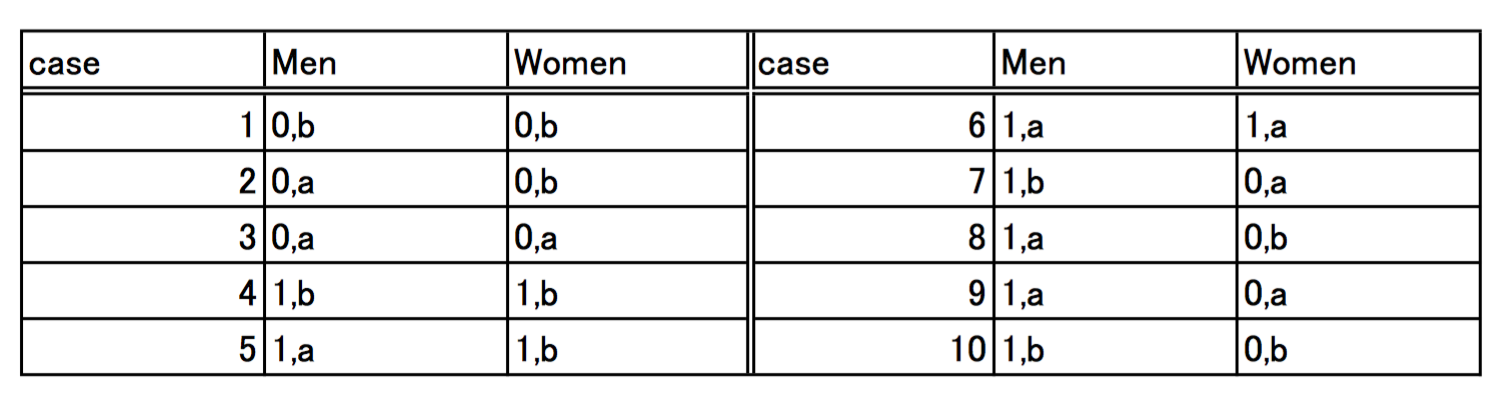
\includegraphics[width = 12cm]{table.png}
\end{center}
\par
These two criterion determine the behavior of the candidates. $1$ leads the strategic thoughts in the same gender group, where $0$ implies that the participants of same gender think the other group members choose them by the same probability. $a$ gives the strategic situation about the choice of partners, where $b$ make the purely probabilistic situation about the choice.
\par
The important point is the definition of the success of this party. I define the success by "all participants can get partners" rather than "the expected number of members getting a partner". This is because almost all participants actually want their one-night stand rather than their companion for life through the party, and so the most essential purpose in the meeting is that all members have so good an experience that they are looking forward to the next party. Thus the success is "all participants can get partners".


\section{Analysis}
	\subsection{No quality gap case}
	\par
	Let A and B be men, and a and b be women. Then each man have two choices, i.e. a or b. And each woman also have two choices, i.e. A or B. In order to summarize the payoff, I write $[\alpha, \beta]$ indicating "$a$ chooses $\alpha$ and $b$ chooses $\beta$ " and $(\alpha, \beta)$ insisting "$A$ chooses $\alpha$ and $B$ chooses $\beta$ ". The payoff matrix can be expressed as Table1, where $x$ is the payoff of getting the partner and $y$ is the payoff of no matching. And $(\alpha, \beta, \gamma, \delta)$ means that $A$ get $\alpha$, $B$ get $\beta$, $a$ get $\gamma$, and $b$ get $\delta$. These notations are used in the below discussion with slight differences.
	\begin{table}[h]
	\begin{center}
                \setlength{\extrarowheight}{2pt}
                \begin{tabular}{*{16}{c|}}
                  \multicolumn{2}{c}{} & \multicolumn{1}{c}{} & \multicolumn{2}{c}{Women}\\\cline{3-6}
                  \multicolumn{1}{c}{} &  & $[A, A]$  & $[A, B]$ & $[B, A]$ & $[B.B]$\\\cline{2-6}
                  \multirow{4}*{Men}  & $(a,a)$ & $(x,y,x,y)$ & $(x,y,x,y)$ & $(y,x,x,y)$ & $(y,x,x,y)$\\\cline{2-6}
                  & $(a,b)$ & $(x,y,x,y)$ & $(x,x,x,x)$ & $(y,y,y,y)$ & $(y,x,y,x)$\\\cline{2-6}
                  & $(b,a)$ & $(x,y,y,x)$ & $(y,y,y,y)$ & $(x,x,x,x)$ & $(y,x,x,y)$\\\cline{2-6}
                  & $(b,b)$ & $(x,y,y,x)$ & $(y,x,y,x)$ & $(x,y,y,x)$ & $(y,x,y,x)$\\\cline{2-6}
                \end{tabular}
        \end{center}
        \caption{no quality gap detting}
  	\end{table}
	\par
	Given the communication skills of members are same, with "Sekigae", all members have the same amount of information about the other sex members. Then, letting $P_\alpha(\beta)$ be the probability of $\alpha$ chooses $\beta$, $P_A(a)= P_B(a) = P_a(A) = P_b(A) = \frac{1}{2}$. Now I consider "no quality gap setting", thenthe decision of each person is independent. In this case, the probability of achieving $\left( (a, b), [A, B] \right)$ or $\left( (b, a), [B, A] \right)$ is $2 \left(\frac{1}{2}\right)^4 = \frac{1}{8}$.
	\par
	Next I consider without "Sekigae" case. I can set the talk pair as "$A - a$" and "$B - b$" without loss of generality and let $\theta$ be the probability gain by longer time talking, i.e. $P_A(a)= P_B(b) = P_a(A) = P_b(B) = \frac{1}{2} + \theta$, where $-\frac{1}{2} \leq\theta \leq \frac{1}{2}$. Because the decision of each person is independent, $P((a,b)) = P([A, B]) = \left( \frac{1}{2} + \theta \right) \left( \frac{1}{2} + \theta\right)$ and $P((b, a)) = P([B, A]) =  \left( \frac{1}{2} - \theta \right) \left( \frac{1}{2} - \theta\right)$. This leads to that the probability of achieving $\left( (a, b), [A, B] \right)$ or $\left( (b, a), [B, A] \right)$ is $ \left( \frac{1}{2} + \theta \right)^4 + \left( \frac{1}{2} - \theta\right)^4 = 2\theta^4 + 3\theta^2 + \frac{1}{8}$.
	Thus the probability of the success is bigger when "Sekigae" is not carried out since $\theta^2$ and $\theta^4 \geq 0$. Furthermore this says that $\theta$ can be negative, or the talk can be used as the tool of giving their own negative impression. And note that I assume that $\theta$ is equal among the pairs.

	\subsection{One side quality gap case}
	$H$ (high quality) and $L$ (low quality) are men. By using the same notation of the previous setting, I can express the payoffs in the Table2, where $x_h$ is the payoff of matching with the high quality man and $x_l$ is one of that with the low quality ($x_h > x_l$).
	
	\begin{table}[h]
		\begin{center}
                \setlength{\extrarowheight}{2pt}
                \begin{tabular}{*{16}{c|}}
                  \multicolumn{2}{c}{} & \multicolumn{1}{c}{} & \multicolumn{2}{c}{Women}\\\cline{3-6}
                  \multicolumn{1}{c}{} &  & $[H, H]$  & $[H, L]$ & $[H, L]$ & $[L.L]$\\\cline{2-6}
                  \multirow{4}*{Men}  & $(a,a)$ & $(x,y,x_h,y)$ & $(x,y,x_h,y)$ & $(y,x,x_l,y)$ & $(y,x,x_l,y)$\\\cline{2-6}
                  & $(a,b)$ & $(x,y,x_h,y)$ & $(x,x,x_h,x_l)$ & $(y,y,y,y)$ & $(y,x,y,x_l)$\\\cline{2-6}
                  & $(b,a)$ & $(x,y,y,x_h)$ & $(y,y,y,y)$ & $(x,x,x_l,x_h)$ & $(y,x,x_l,y)$\\\cline{2-6}
                  & $(b,b)$ & $(x,y,y,x_h)$ & $(y,x,y,x_l)$ & $(x,y,y,x_h)$ & $(y,x,y,x_l)$\\\cline{2-6}
                \end{tabular}
                \end{center}
                \caption{difference vs no difference}
          \end{table}
          
          \par
          With "Sekigae", all men put the same probability on each choice, i.e. $P_H(a) = P_L(a) = \frac{1}{2}$. Then all rows in the Table2 happen with a probability of quarter 1. In this situation the payoff matrix of the women side can be expressed as Table3 due to the calculation of the expected value from Table2.

	\begin{table}[h]
		\begin{center}
		\begingroup
                \renewcommand{\arraystretch}{1.5}
                \setlength{\extrarowheight}{2pt}
                \begin{tabular}{*{4}{c|}}
                  \multicolumn{2}{c}{} & \multicolumn{2}{c}{b}\\\cline{3-4}
                  \multicolumn{1}{c}{} &  & $H$  & $L$ \\\cline{2-4}
                  \multirow{2}*{a}  & $H$ & $(\frac{x_h+y}{2}, \frac{x_h+y}{2})$ & $(\frac{x_h+y}{2}, \frac{x_l+y}{2})$ \\\cline{2-4}
                  & $L$ & $(\frac{x_l+y}{2}, \frac{x_h+y}{2})$ & $(\frac{x_l+y}{2}, \frac{x_l+y}{2})$ \\\cline{2-4}
                \end{tabular}
                \endgroup
                \end{center}
                \caption{women's payoff matrix with Sekigae}
  	\end{table}
	
	\par
	Since $x_h > x_l$, $H$ is a strictly dominant strategy for both $a$ and $b$. This means that $[H, H]$ is realized in figure 2 and  two matchings can never be achieved in this case.
	\par
	Next I consider no "Sekigae" case. Let the talk pair be "$H - a$" and "$L - b$" without loss of generality and $\theta$ be the probability gain by the longer talks ($-\frac{1}{2} \leq \theta \leq \frac{1}{2}$). Given that $P_H(a) = P_L(b) = \frac{1}{2} + \theta$, women side have the payoff matrix expressed in Table4.

	\begin{table}[h]
                \begin{center}
                \begingroup
                \renewcommand{\arraystretch}{1.8}
                \begin{tabular}{*{4}{c|}}
                  \multicolumn{2}{c}{} & \multicolumn{2}{c}{b}\\\cline{3-4}
                  \multicolumn{1}{c}{} &  & $H$  & $L$ \\\cline{2-4}
                  \multirow{2}*{a}  & $H$ & $((x_h - y)\theta + \frac{x_h+y}{2}, (y - x_h)\theta + \frac{x_h+y}{2})$ & $((x_h - y)\theta+\frac{x_h+y}{2}, (x_l - y)\theta + \frac{x_l+y}{2})$ \\\cline{2-4}
                  & $L$ & $((y-x_l)\theta + \frac{x_l+y}{2}, (y-x_h)\theta + \frac{x_h+y}{2})$ & $((y-x_l)\theta + \frac{x_l+y}{2}, (x_l - y)\theta + \frac{x_l+y}{2})$ \\\cline{2-4}
                \end{tabular}
                \endgroup
                \end{center}
                \caption{women's payoff matrix without Sekigae}
  	\end{table}
	
	\par
	For example, I calculate the payoffs of the case in which both $a$ and $b$ choose $H$.
	\begin{align*}
	\text{a's payoff} = (\frac{1}{2} + \theta)(\frac{1}{2} - \theta)x_h + (\frac{1}{2} + \theta)(\frac{1}{2} + \theta)x_h + (\frac{1}{2} - \theta)(\frac{1}{2} - \theta)y + (\frac{1}{2} - \theta)(\frac{1}{2} + \theta)y = (x_h - y)\theta + \frac{h_h + y}{2} \\[10pt]
	\text{b's payoff} = (\frac{1}{2} + \theta)(\frac{1}{2} - \theta)y + (\frac{1}{2} + \theta)(\frac{1}{2} + \theta)y + (\frac{1}{2} - \theta)(\frac{1}{2} - \theta)x_h + (\frac{1}{2} - \theta)(\frac{1}{2} + \theta)x_h = (y - x_h)\theta + \frac{h_h + y}{2}
	\end{align*}
	the rest of all components in Table4 can be calculated by the same way.
	\par
	For simplicity let $\theta > 0$. And I assume that $x_h > x_l > y$. This is the key assumption. Now H strictly dominates L for a by the assumption. Thus if b's payoff of choosing L is bigger than one of H, $[H, L]$ can be achieved. The condition is as follows.
	\begin{align*}
	&\qquad (x_l - y)\theta + \frac{x_l + y}{2} - \left\{ (y - x_h)\theta + \frac{x_h + y}{2} \right\} > 0\\
	&\Leftrightarrow (x_h + x_l - 2y)\theta + \frac{x_l - x_h}{2} > 0\\[8pt]
	&\Leftrightarrow \theta > \frac{x_h - x_l}{2} \frac{1}{x_h + x_l - 2y}
	\end{align*}
	The last line is due to the $x_h > x_l > y$. And this assumption allows $\frac{x_h - x_l}{2} \frac{1}{x_h + x_l - 2y}$ to be less than $\frac{1}{2}$.
	\par
	If this condition of $\theta$ can be achieved, the probability of matching all members is the probability of "H chooses a and L chooses b". Now I get the below.
	\begin{align*}
	P((a, b)) = (\frac{1}{2} + \theta)^2
	> \left( \frac{1}{2} + \frac{x_h - x_l}{2} \frac{1}{x_h + x_l - 2y} \right)^2
	= \left( \frac{x_h - y}{x_h + x_l -2y} \right)
	= \left( \frac{1}{1 + \frac{x_l - y}{x_h -y}}\right)
	\end{align*}
	The above shows that the lower bound of the probability of success is the decreasing function of $\frac{x_l - y}{x_h - y}$. And this is the increasing function of $x_h$. Then in this one side gap setting "Sekigae" should not be carried out. And the bigger gap among one group exists, the more likely all members get their own partners.
	\par
	Let's compare the result with the no gap situation.
	\begin{align*}
	\left( 2\theta^4 + 3\theta^2 + \frac{1}{8} \right) - \left( \theta + \frac{1}{2} \right)^2 < 0\\
	\Leftrightarrow -0.10339 \dots < \theta < \frac{1}{2}
	\end{align*}
	This means that one side gap setting gives the bigger probability of success than no gap setting if $\frac{1}{2} > \theta > \frac{x_h - x_l}{2} \frac{1}{x_h + x_l - 2y}$ and "Sekigae" is not carried out.
	
	\subsection{Two side quality gap case}
	In this case, all the players know which of the other group members is high quality or low quality and know that among their own group. This is a highly strategic situation. The payoffs are summarized in figure 5, where $x_h$ is the payoff for matching with a high quality person and $x_l$ is one with a low quality person ($x_h > x_l$). I assume that $x_l > y$. This is the same assumption in the previous setting and plays a big roll. Note that $[\alpha, \beta]$ means "high quality woman chooses $\alpha$ quality man and low quality woman chooses $\beta$ quality man". The same notation is used for $(\alpha, \beta)$.
	
	\begin{table}[h]
	\begin{center}
                \setlength{\extrarowheight}{2pt}
                \begin{tabular}{*{16}{c|}}
                  \multicolumn{2}{c}{} & \multicolumn{1}{c}{} & \multicolumn{2}{c}{Women}\\\cline{3-6}
                  \multicolumn{1}{c}{} &  & $[H, H]$  & $[H, L]$ & $[H, L]$ & $[L.L]$\\\cline{2-6}
                  \multirow{4}*{Men}  & $(h,h)$ & $(x_h,y,x_h,y)$ & $(x_h,y,x_h,y)$ & $(y,x_h,x_l,y)$ & $(y,x_h,x_l,y)$\\\cline{2-6}
                  & $(h,l)$ & $(x_h,y,x_h,y)$ & $(x_h,x_l,x_h,x_l)$ & $(y,y,y,y)$ & $(y,x_l,y,x_l)$\\\cline{2-6}
                  & $(l,h)$ & $(x_l,y,y,x_h)$ & $(y,y,y,y)$ & $(x_l,x_h,x_l,x_h)$ & $(y,x_h,x_l,y)$\\\cline{2-6}
                  & $(l,l)$ & $(x_l,y,y,x_h)$ & $(y,x_l,y,x_l)$ & $(x_l,y,y,x_h)$ & $(y,x_l,y,x_l)$\\\cline{2-6}
                \end{tabular}
        \end{center}
        \caption{difference vs difference}
  	\end{table}

	\par
	First I consider "Sekigae" case and assume that all people in this model think "High quality persons match high quality one". I introduce this assumption as an idea accepted in common in order to study the success. This assumption make the payoff matrix very simple as in table 6.
	
	\begin{table}[h]
	\begin{center}
                \setlength{\extrarowheight}{2pt}
                \begin{tabular}{*{4}{c|}}
                  \multicolumn{2}{c}{} & \multicolumn{2}{c}{l}\\\cline{3-4}
                  \multicolumn{1}{c}{} &  & $H$  & $L$ \\\cline{2-4}
                  \multirow{2}*{L}  & $h$ & $(y,y)$ & $(y,y)$\\\cline{2-4}
                  & $l$ & $(y,y)$ & $(x_l, x_l)$ \\\cline{2-4}
                \end{tabular}
        \end{center}
        \caption{payoff matrix for the low quality persons}
  	\end{table}
	
	\par
	Let $x_h > x_l > y$.
	This matrix is the left upper part of table 5. And in this situation choosing the low quality dominates the other choice for both of them. Then $((h, l), [H, L])$ is always achieved as a whole. This means the probability of two matching is 1. Furthermore I get the same result under another assumption, which is "Low quality persons can not match with High quality persons, so should choose Low quality persons". In this situation The payoff matrix can be simplified like the previous one and choosing high quality dominates choosing low quality for the two high quality participants. Then $((h, l), [H, L])$ is always realized.
	\par
	In no "Sekigae" case, I write the payoff gain from the longer time of talking as $\tau$, but it ends up to the same result under the common idea assumptions provided in the previous setting however $\tau$ is large. Thus next I relieve the assumption and consider the general case equilibriums. But I only consider the case with "Sekigae" due to the words restriction.
	\par
	I derive the mixed strategy Nash equilibrium in "Sekigae" case. Let $P_\alpha(\beta)$ be the probability that $\alpha$ chooses $\beta$. And denote $P_H(h) = a, P_L(h) = b, P_h(H) = c, P_l(H) = d$. Then the expected payoff of $H$ when he chooses $h$ is as follows. 
	\begin{align}
	&bcdx_h + bc(1-d)x_h + b(1-c)dy + b(1-c)(1-d)y \nonumber \\&+ (1-b)cdx_h + (1-b)c(1-d)x_h + (1-b)(1-c)dy + (1-b)(1-c)(1-d)y
	\end{align}
	When he chooses $l$, the payoff is as follows.
	\begin{align}
	&bcdx_l + bc(1-d)y + b(1-c)dx_l + b(1-c)(1-d)y \nonumber \\&+ (1-b)cdx_l + (1-b)c(1-d)y + (1-b)(1-c)dx_l + (1-b)(1-c)(1-d)y
	\end{align}
	these can be calculated from table 5. Now the border between the two choices is 
	\begin{align}
	(1) - (2) &=  cd(x_h - x_l) + c(1-d)(x_h - y) + (1-c)d(y - x_l) \nonumber \\
	&= cd(x_h - x_l - x_h + y -y + x_l) + c(x_h - y) + d(y - x_l) \nonumber\\
	&= c(x_h - y) + d(y - x_l) = 0 \nonumber\\
	&\Leftrightarrow \frac{c}{d} = \frac{x_l - y}{x_h - y}
	\end{align}
	The same logic can be used for $L$ case. Thus I omit the detail and get the below border.
	\begin{align}
	&c(1 - d)(y - x_l) + (1 - c)d(x_h - y) + (1-c)(1-d)(x_h - x_l) \nonumber \\
	&= cd(x_l - y + y -x_h + x_h - x_l) + c(y - x_l) + d(x_h - y) + (x_h - x_l) - c(x_h - x_l) - d(x_h - x_l)\nonumber \\
	&= c(y - x_h) + d(x_l - y) + (x_h - y) + (y - x_l) = (x_h - y)(1 - c) + (y - x_l)(1 - d) = 0 \nonumber \\
	&\Leftrightarrow \frac{1-c}{1-d} = \frac{x_l - y}{x_h - y}
	\end{align}
	Then I get the best response function about $a$ and $b$ as follows.
	\begin{align*}
            	\begin{cases}
            	a = 1, b= 0 & \left( \frac{x_l - y}{x_h - y}(d-1) + 1 < c \leq 1 \right) \\[8pt]
            	a = 1, 0 \leq b \leq 1 & \left( c = \frac{x_l - y}{x_h - y}(d-1) + 1 \right) \\[8pt]
		a = 1, b = 1 & \left( \frac{x_l - y}{x_h - y}d < c < \frac{x_l - y}{x_h - y}(d-1) + 1 \right) \\[8pt]
		0 \leq a \leq 1, b = 1 & \left( c = \frac{x_l - y}{x_h - y}d \right) \\[8pt]
		a = 0, b = 1 & \left( 0 \leq c < \frac{x_l - y}{x_h - y}d \right)
            	\end{cases}
	\end{align*}
	And the same logic is applied to calculate the best response function about $c$ and $d$.
	\begin{align*}
            	\begin{cases}
            	c = 1, d= 0 & \left( \frac{x_l - y}{x_h - y}(b-1) + 1 < a \leq 1 \right) \\[8pt]
            	c = 1, 0 \leq d \leq 1 & \left( a = \frac{x_l - y}{x_h - y}(b-1) + 1 \right) \\[8pt]
		c = 1, d = 1 & \left( \frac{x_l - y}{x_h - y}b < a < \frac{x_l - y}{x_h - y}(b-1) + 1 \right) \\[8pt]
		0 \leq c \leq 1, d = 1 & \left( a = \frac{x_l - y}{x_h - y}b \right) \\[8pt]
		c = 0, d = 1 & \left( 0 \leq a < \frac{x_l - y}{x_h - y}b \right)
            	\end{cases}
	\end{align*}
	The mixed strategy Nash equilibriums are the the pairs of the probabilities which respond mutually best. Thus There are 4 mixed strategy Nash equilibriums by the above best response functions.
	\begin{align}
	&(a = 1, b = 0, c = 1, d = 0)\\
	&(a = 1, b = 1, c =1, d = 1)\\
	&\left(a = \frac{x_l - y}{x_h - y}, b = 1, c = \frac{x_l - y}{x_h - y}, d = 1 \right)\\
	&(a = 0, b = 1, c = 0, d = 1)
	\end{align}
	If each of these four equilibriums are realized by the same probability ($\frac{1}{4}$ for each), the probability of two pair matching is $P = \frac{1}{4} + \frac{1}{4} + \left( 1 - \frac{x_l - y}{x_h - y} \right)^2$, which is a increasing function about $x_h$. And $P \to \frac{3}{4}$ as $x_h \to \infty$.

\section{Conclusion}
\par
In this paper I study the strategic characteristics of Japanese singles party, particularly considering "no quality gap setting", "one side quality gap setting" and "two side quality gap setting". These settings are three from the cases which are classified by the recognition of quality gap in the participants own group and by the common knowledge in each sex group about the quality gap in the other group. 
\par
I show that no "Sekigae" situation is better than with "Sekigae" except the two side quality gap setting. And one side quality gap setting can give the bigger probability of two pair matching than no quality gap setting. Furthermore I clarify the importace of assuming that $x_l > y$. That is, it is essential in Japanese singles party for all members to prefer matching with any participant in the other group to matching with nobody.
Another finding is that the probability of two pair matching is a increasing function about $x_h$ in both one side quality gap setting and two side quality gap setting.
Thus there are two important points to get a success in the meeting, which are having so-so members for both groups and at least one of them in each group being extremely high quality person.
\par
Finally I mention the further study direction. First is calculating the mixed strategy Nash equilibrium of two side quality gap setting without "Sekigae" and analyzing the characteristics. Next is extending this model to the dynamic one. These parties are typically planned by one man and one woman, each of who is the leader of each group. They gather the each sex participants and make a decision whether "Sekigae" is carried out or not. This means that they can choose the quality in each group and manipulate the talk time. Furthermore these two persons can take contact with each other in advance to make the party better for them. These dynamic situation must reveal the more interesting part of this party.

\begin{thebibliography}{9}
\bibitem{Okada} Akira Okada, "Game Theory, " Japan, Oct, 2014
\end{thebibliography}

\end{document}



















